\documentclass[15 pt,]{article}
\usepackage{lmodern}
\usepackage{amssymb,amsmath}
\usepackage{ifxetex,ifluatex}
\usepackage{fixltx2e} % provides \textsubscript
\ifnum 0\ifxetex 1\fi\ifluatex 1\fi=0 % if pdftex
  \usepackage[T1]{fontenc}
  \usepackage[utf8]{inputenc}
\else % if luatex or xelatex
  \ifxetex
    \usepackage{mathspec}
  \else
    \usepackage{fontspec}
  \fi
  \defaultfontfeatures{Ligatures=TeX,Scale=MatchLowercase}
\fi
% use upquote if available, for straight quotes in verbatim environments
\IfFileExists{upquote.sty}{\usepackage{upquote}}{}
% use microtype if available
\IfFileExists{microtype.sty}{%
\usepackage{microtype}
\UseMicrotypeSet[protrusion]{basicmath} % disable protrusion for tt fonts
}{}
\usepackage[margin=1in]{geometry}
\usepackage{hyperref}
\hypersetup{unicode=true,
            pdftitle={Fit a misspecified model with measurement error using CCP},
            pdfauthor={Tianying Wang},
            pdfborder={0 0 0},
            breaklinks=true}
\urlstyle{same}  % don't use monospace font for urls
\usepackage{graphicx,grffile}
\makeatletter
\def\maxwidth{\ifdim\Gin@nat@width>\linewidth\linewidth\else\Gin@nat@width\fi}
\def\maxheight{\ifdim\Gin@nat@height>\textheight\textheight\else\Gin@nat@height\fi}
\makeatother
% Scale images if necessary, so that they will not overflow the page
% margins by default, and it is still possible to overwrite the defaults
% using explicit options in \includegraphics[width, height, ...]{}
\setkeys{Gin}{width=\maxwidth,height=\maxheight,keepaspectratio}
\IfFileExists{parskip.sty}{%
\usepackage{parskip}
}{% else
\setlength{\parindent}{0pt}
\setlength{\parskip}{6pt plus 2pt minus 1pt}
}
\setlength{\emergencystretch}{3em}  % prevent overfull lines
\providecommand{\tightlist}{%
  \setlength{\itemsep}{0pt}\setlength{\parskip}{0pt}}
\setcounter{secnumdepth}{0}
% Redefines (sub)paragraphs to behave more like sections
\ifx\paragraph\undefined\else
\let\oldparagraph\paragraph
\renewcommand{\paragraph}[1]{\oldparagraph{#1}\mbox{}}
\fi
\ifx\subparagraph\undefined\else
\let\oldsubparagraph\subparagraph
\renewcommand{\subparagraph}[1]{\oldsubparagraph{#1}\mbox{}}
\fi

%%% Use protect on footnotes to avoid problems with footnotes in titles
\let\rmarkdownfootnote\footnote%
\def\footnote{\protect\rmarkdownfootnote}

%%% Change title format to be more compact
\usepackage{titling}

% Create subtitle command for use in maketitle
\newcommand{\subtitle}[1]{
  \posttitle{
    \begin{center}\large#1\end{center}
    }
}

\setlength{\droptitle}{-2em}
  \title{Fit a misspecified model with measurement error using CCP}
  \pretitle{\vspace{\droptitle}\centering\huge}
  \posttitle{\par}
  \author{Tianying Wang}
  \preauthor{\centering\large\emph}
  \postauthor{\par}
  \predate{\centering\large\emph}
  \postdate{\par}
  \date{2018-06-25}

\usepackage{color}

\begin{document}
\maketitle

\newcommand{\bomega}{\mbox{\boldmath $\omega$}}
\newcommand{\bbeta}{\mbox{\boldmath $\beta$}}
\newcommand{\bTheta}{\mbox{\boldmath $\Theta$}}
\newcommand{\bOmega}{\mbox{\boldmath $\Omega$}}
\newcommand{\bLambda}{\mbox{\boldmath $\Lambda$}}

\def\extLambda{\bLambda_{\rm ext}} \def\intLambda{\bLambda_{\rm int}}
\def\sumi{\hbox{$\sum_{i=1}^{n}$}} \def\sumj{\hbox{$\sum_{j=1}^J$}}
\def\suml{\hbox{$\sum_{\ell=1}^L$}}
\def\sumk{\hbox{$\sum_{k=1}^{K_{\ell}}$}}
\def\sumkl{\hbox{$\sum_{k,\ell}$}} \def\sumb{\hbox{$\sum_{b=1}^{B}$}}
\def\exPhi{\Phi_{\rm true}} \def\catPhi{\Phi_{\rm cat}}
\def\wh{\widehat} \def\trans{^{\rm T}} \def\pr{\hbox{pr}}

\section{Abstract}\label{abstract}

This document provides further details and a concrete illustration for
the R programs used in the paper \emph{Categorizing a Continuous
Predictor Subject to Measurement Error} (Blas et al. 2018+). This
package is mainly focused on logistic regression and linear regression,
though the proposed method has much weaker assumptions and can be
applied in many scenarios. This document provides a brief overview of
the methodology, especially for linear regression and logistic
regression. Further, we use simulation studies and a real data example,
the EATS data (Subar et al. 2001), to show 4 ways to use \texttt{ccp},
the main function in the \texttt{CCP} package.

\section{Introduction}\label{introduction}

In epidemiology, it is common to fit a categorical risk model to a
continuous risk predictor, because the categorical one is thought to be
more robust and interpretable. When the risk predictor is observed with
measurement error, epidemiologists typically ignore the underlying
measurement error and perform a naive approach, e.g., logistic
regression, as what they would have done if they observe the true
predictor. Here we introduce some notation to help describe the problem
background.

\begin{itemize}
\tightlist
\item
  \(X\): true risk predictor (continuous);
\item
  \(X_{\rm C}\): categorized predictor;
\item
  \(U\): measurement error;
\item
  \(W\): observed risk predictor (continuous, with measurement error);
  \(W = X + U\), \(X\) and \(U\) are independent;
\item
  \(W_{\rm C}\): categorized predictor.
\end{itemize}

Using the notation stated above, ideally, epidemiologists categorize
\(X\) and then use \(X_{\rm C}\) to fit the model. However, if they
observe \(W\) instead of \(X\), they would use \(W_{\rm C}\) in the
original categorical model without correcting the measurement error.

White (1982) shows that when \(X\) is observed, though the categorical
model is a misspecified model, the estimates are unbiased with respect
to the true value of what epidemiologists are interested in - the
parameters with respect to \(X_C\) in the categorical risk model. When
\(X\) is not observed, however, substituting \(W\) for \(X\) leads to a
biased estimate, as well as a poor inference quality. To address the
problem based on \(W\), the relationship between \(W\) and \(X\) needs
to be specified.

We address this problem and provide a general method to get unbiased
estimates and correct inference even with measurement error in the data.
The key of our method is adding another layer of conditional expectation
given observed predictor \(W\). Thus, the original estimating equation
is now relying on \(W\) but not on \(X\). We then need to estimate the
expectations of functions of \(X\) given \(W\). For example, suppose the
original estimating equation is formed based on \(E\{f(X)\} = 0\).
Adding a layer of conditional expectation leads to \(E[E\{f(X)|W\}]=0\).
Hence, the goal turns out to be estimating \(E\{f(X)|W\}\), depending on
the conditional density \(f_{X|W}\). Although Blas et al. (2018+)
focuses on the general case, this document aims to provide more details
for logistic regression and linear regression.

Due to the complexity of the problem itself, in this package, we do not
consider other covariates measured without error. Readers can find more
general formulas in the original paper.

The rest of this document is organized as follows: we first provide a
brief methodology review for readers to gain more background without
looking at the original paper; then, we present estimating equations in
logistic regression and linear regression. Finally, we show different
ways to use the main function \texttt{ccp} through simulation studies,
as well as the analysis for EATS data (Subar et al. 2001).

\section{Methodology review}\label{methodology-review}

\subsection{General overview}\label{general-overview}

Here we present two cases: linear regression and logistic regression,
corresponding to continuous or binary response. For the more general
model and its assumptions, we refer readers to \emph{Categorizing a
Continuous Predictor} for more details.

This package allows users to use two types of data:

\begin{itemize}
\item
  External-internal data: if the main dataset has no replicates, users
  need to provide external data for nuisance parameter estimation,
  especially for estimating the variance of measurement error. Without
  external data, the measurement error is unidentifiable.
\item
  Internal-only data: when the main dataset has replicates, the program
  only uses the main dataset to calculate the nuisance parameters. Any
  provided external data are ignored in this case.
\end{itemize}

In the following part, we explain the external-internal and
internal-only cases in linear regression and logistic regression,
respectively.

In the R package \texttt{CCP}, we assume that \[
                        W= X + U; \hskip 5mm
                        X \sim N(\mu_x,\sigma_x^2); \hskip 5mm
                        U \sim N(0,\sigma^2_u).
                    \] Also, \(X\) and \(U\) are independent. For
convenience, we define nuisance parameter
\(\bLambda = (\mu_x, \sigma^2_x, \sigma^2_u)\).

For the continuous risk predictor \(X\), we denote
\(m(X, \bbeta) = \alpha + X \beta\), where
\(\bbeta = ( \alpha, \beta)\). To categorize \(X\) into \(j = 1,..., J\)
categories \((C_1, ..., C_J)\), we define
\(M(X) = \{ I(X\in C_1),..., I(X\in C_J)\}\trans\). Thus, the
corresponding parameters in the categorical model are
\(\bTheta = (\theta_1,..., \theta_J)\).

The parameter we are mainly interested in is \(\theta_J - \theta_1\),
which is the \emph{log relative risk} in logistic regression.

Now we introduce three assumptions required for our approach:

\begin{enumerate}
\def\labelenumi{(\alph{enumi})}
\item
  When \(X\) is observed, the true risk model in the continuous scale
  has unbiased estimating functions known up to parameters \(\bbeta\).
\item
  When \(X\) is not observed, we can find a function \(g(X, \bbeta)\)
  that \(E[E\{g(X, \bbeta)|W\}]=0\), with its conditional expectation
  \(E\{g(X, \bbeta)|W\}\) depends on \(\bLambda\) and can be estimated.
  A special case is knowing the distribution of \(X\) given \(W\) up to
  parameters \(\bLambda\).
\item
  If the external data are necessary for model identification, the
  parameter estimated from external data, i.e. \(\sigma^2_u\), should be
  transportable. See Chapter 2.2.4-2.2.5 of R. J. Carroll et al. (2006).
\end{enumerate}

For linear regression and logistic regression considered in this
package, all three assumptions are satisfied. Further, we would like to
point out that neither normally distributed \(X\) and \(U\), nor
logistic or linear regression model is specifically required for the
proposed method itself.

To estimate nuisance parameters \(\bLambda\), we now introduce the
estimating equations based on using external-internal or internal-only
data. Then the estimating equations for \(\bbeta\) and \(\bTheta\) are
introduced, depending on using linear regression or logistic regression.

\subsubsection{External-internal data}\label{external-internal-data}

If there are no replicates in the internal data, we use the external
data only to estimate \(\sigma_u^2\). Suppose we observe
\(W_{ik} = X_i + U_{ik}\) for \(k=1,...,K\) and \(i=n+1,...,n+N\). We
use internal data to estimate \(\mu_x,\sigma^2_x\) without replicates.

In the external data, let
\(\overline{W}_{i\cdot} = K^{-1} \sum_{k=1}^{K}W_{ik}\). Define
\(\wh{\sigma}^2_{u,i} = (K-1)^{-1} \sum_{k=1}^K (W_{ik} - \overline{W}_{i\cdot})^2\)
to be the sample variance of the \(W_{ik}\) for a given \(i\).

Because \(E\{ (W_{i} - \mu_x)^2\} = \sigma_x^2 + \sigma_u^2\), unbiased
estimating equations for \(\bLambda=(\mu_x,\sigma^2_x,\sigma^2_u)\) are

\begin{itemize}
\item
  For \(\mu_x\): \(n^{-1} \sumi (W_i - \mu_x)=0\);
\item
  For \(\sigma_u^2\):
  \(N^{-1}\sum_{i=n+1}^{n+N} (\wh{\sigma}^2_{u,i} - \sigma_u^2)=0\).
\item
  For \(\sigma_x^2\):
  \(n^{-1} \sumi \{ (W_i - \mu_x)^2 - \sigma_x^2 - \sigma_u^2\}=0\);
\end{itemize}

\subsubsection{Internal-only data}\label{internal-only-data}

Suppose there are no external data, and we have replicates \(W_{ir}\)
for \(r= 1,...,R\) in the internal data. Now we use the internal data to
estimate \(\Lambda =(\mu_x,\sigma_x^2,\sigma_{uR}^2)\), and we observe
\(W_{ir} = X_i + U_{ir}\) for \(r=1,...,R\) and \(i=1,...,n\). Define
\(\overline{W}_{i\cdot} = R^{-1}\sum_{r=1}^R W_{ir}\). Define
\(\wh{\sigma}^2_{u,i}\) to be the sample variance of the \(W_{ir}\)
within subject \(i\), and define \(\sigma_u^2/R = \sigma^2_{uR}\).The
estimating equations are

\begin{itemize}
\item
  For \(\mu_x\): \(n^{-1} \sumi (\overline{W}_{i\cdot} - \mu_x)=0\);
\item
  For \(\sigma_{uR}^2\):
  \(n^{-1}\sumi (\wh{\sigma}^2_{u,i}/R - \sigma_{uR}^2)=0\).
\item
  For \(\sigma_x^2\):
  \(n^{-1} \sumi \{ (\overline{W}_{i\cdot} - \mu_x)^2 - \sigma_x^2 - \sigma_{uR}^2\}=0\);
\end{itemize}

Using the external-internal or internal-only data influences how to
estimate nuisance parameters \(\bLambda\), while fitting linear or
logistic regression affects the estimating equations of
\(\bbeta, \bTheta\) as described below.

\subsection{Linear regression}\label{linear-regression}

We assume the true model in the continuous scale is\[
                        Y  = \alpha + X \beta+\epsilon =  m(X, \bbeta) + \epsilon,\]
where \(m(X, \bbeta) = \alpha + X\beta.\) For external-internal and
internal-only cases, the estimation equations for \(\bbeta\) and
\(\bTheta\) are the same.

The estimating function for \(\bbeta=(\alpha,\beta)\) is \[
\Phi ( \bbeta,\wh\bLambda) = n^{-1}\sumi E[\{Y_i - m(X_i, \bbeta) \}\partial m(X_i, \bbeta) / \partial\bbeta\trans  \vert W_i ].
\] The estimating function for \(\bTheta\) is \[
Q(W_i,\bTheta, \wh\bbeta,\wh\bLambda)  =  E \left[\begin{array}{c}
m(X_i,\wh\bbeta) I(X_i \in C_1) - \bTheta_1 I(X_i \in C_1) \\
\vdots \\
m(X_i,\wh\bbeta) I(X_i \in C_J) - \bTheta_J I(X_i \in C_J)
\end{array} \vline \hbox{ } W_i \right].
\] The integration above is calculated using the \texttt{integrate}
function in the R package \texttt{stats}.

\subsection{Logistic regression}\label{logistic-regression}

Let \(H(\cdot)\) denote the logistic distribution function. Here we
consider the special case of linear logistic regression with the
classical measurement error model in both the external and internal
datasets: \[
                \pr(Y = 1 \vert X,Z) = H(\alpha + X\beta) =   H\{(1, X)\bbeta\}\]

Let
\(p_i = \pr(Y=1 \vert W_i) = \int H\{(1, x)\bbeta\} f_{x\vert W_i}(x,W_i,\bLambda) dx\),
we use the \texttt{integrate} function in the R package \texttt{stats}
to compute this quantity and calculate the loglikelihood
\(\propto n^{-1}\sumi Y_i\log(p_i)+(1-Y_i)\log(1-p_i)\). We then use the
\texttt{optim} function in the R package \texttt{stats} to minimize
negative loglikelihood to estimate \(\bbeta\).

Given the logistic regression model, the categorical estimating function
is \[
                \catPhi\{Y,M\trans(X)\bTheta\} = M(X) [Y - H\{M\trans(X)\bTheta\}],
\] Where \(M(X) = \{ I(X\in C_1),..., I(X\in C_J)\}\trans\) for
categories \((C_1, ..., C_J)\). Hence, with
\(\bOmega = (\bTheta,\bbeta,\bLambda)\), \[
                Q(W,\bOmega) = E\left( M(X) \left[H\{m(X, \bbeta)\} - H\{M\trans (X)\bTheta\}\right]\bigg\vert W\right).
                \] In the R program,

\begin{equation*}
Q(W_i,\bTheta, \wh\bbeta,\wh\bLambda)  =  E \left[\begin{array}{c}
H\{m(X_i, \wh\bbeta)\} I(X_i \in C_1) - H(\bTheta_1) I(X_i \in C_1) \\
\vdots \\
H\{m(X_i, \wh\bbeta)\} I(X_i \in C_J) - H(\bTheta_J) I(X_i \in C_J)
\end{array} \vline \hbox{ } W_i \right].
\end{equation*}

Again, we use the \texttt{integrate} function in the R package
\texttt{stats} to compute the integrals.

\section{Function overview}\label{function-overview}

\begin{figure}

{\centering 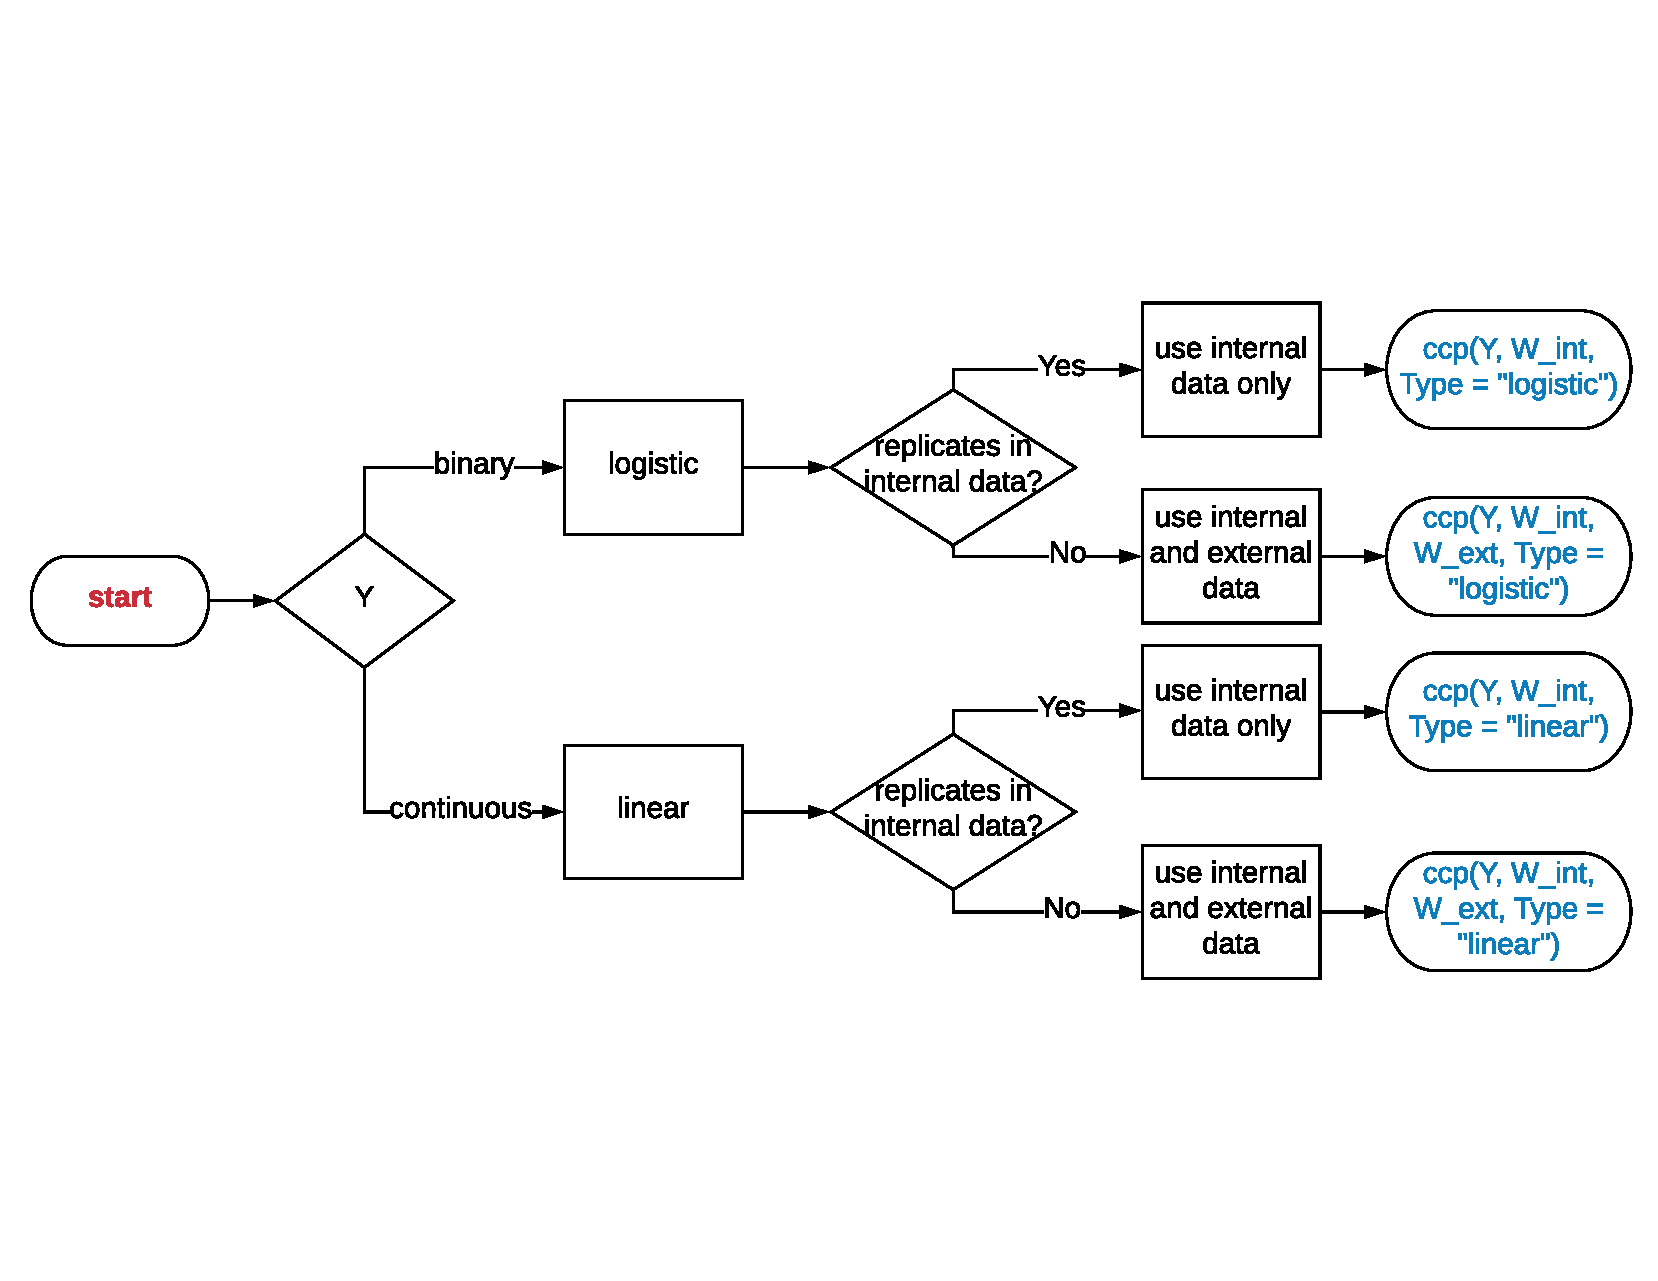
\includegraphics[width=0.95\linewidth]{CCP} 

}

\caption{Functions overview}\label{fig:unnamed-chunk-1}
\end{figure}

As shown in Figure 1, the package \texttt{CCP} contains one main
function named `ccp'. Based on the types of response, we can specify
logistic regression for binary \(Y\), or linear regression for
continuous \(Y\). Further, in each of the two cases we mentioned before,
\texttt{ccp} provides the choice of external-internal and internal-only
cases as introduced in the methodology review.

\subsection{Get started}\label{get-started}

First, let us install the R package \texttt{CCP}.

\begin{verbatim}
install.packages("~/Desktop/CCP_1.1.tar.gz", repos = NULL, type = "source")
#> Warning in install.packages("~/Desktop/CCP_1.1.tar.gz", repos = NULL,
#> type = "source"): installation of package '/Users/tianying/Desktop/
#> CCP_1.1.tar.gz' had non-zero exit status
library(CCP)
\end{verbatim}

Once the package has been loaded, one can call the main function as
follows.

\begin{verbatim}
ccp(y, W_int, W_ext = NULL, C = NULL, Type, print.summary = TRUE, standardize = TRUE)
\end{verbatim}

To check the package \texttt{CCP} or the usage of a specific function,
you can either use \texttt{help} or \texttt{??}.

\begin{verbatim}
help( package = "CCP" )
??ccp
\end{verbatim}

The former command gives a brief summary of all functions in the
package, while the later one offers more detailed information for
function \texttt{ccp}.

\section{Simulation study}\label{simulation-study}

Here we show the external-internal and internal-only cases for logistic
regression. We also compare the proposed method with the naive approach:
substituting \(W\) for \(X\) in the categorical model with no adjustment
for measurement error.

\begin{enumerate}
\def\labelenumi{(\arabic{enumi})}
\tightlist
\item
  Define a function to calculate the naive estimates.
\end{enumerate}

\begin{verbatim}
thetaw <- function(y, w, mux_hat, s2x_hat){
  
  # Define cut points
  
  J = 5 # categorize W into quintiles
  C = rep(0, 4)
  C[1] = qnorm(0.2, mean = mux_hat, sd = sqrt(s2x_hat))
  C[2] = qnorm(0.4, mean = mux_hat, sd = sqrt(s2x_hat))
  C[3] = qnorm(0.6, mean = mux_hat, sd = sqrt(s2x_hat))
  C[4] = qnorm(0.8, mean = mux_hat, sd = sqrt(s2x_hat))
  
  # Define a function to categorize W
  fMx <- function(x){
    Mx = vector()
    Mx[1] = ifelse(x < C[1], 1, 0)
    Mx[2] = ifelse((C[1] <= x) & (x < C[2]), 1, 0)
    Mx[3] = ifelse((C[2] <= x) & (x < C[3]), 1, 0)
    Mx[4] = ifelse((C[3] <= x) & (x < C[4]), 1, 0)
    Mx[5] = ifelse(x >= C[4], 1, 0)
    return (Mx)
  }  
  
# Categorize W
cw = matrix(0, ncol = J,nrow = n)
for(i in 1:n){cw[i, ] = fMx(w[i])}

# Run standard logistic regression using glm (no intercept)
thetaw_out = glm(y ~ cw - 1 , family = binomial(link = "logit"))

# Get estimates theta1, .., that_5 and standard errors
thetaw_w = summary(thetaw_out)$coef[1:J] 
s.e.thw = summary(thetaw_out)$coef[1:J, 2]

# Calculate the standard error for theta_5 - theta_1
s.e_thetaw_J1 = sqrt(s.e.thw[J]^2+s.e.thw[1]^2 -2*vcov(thetaw_out)[1,J])
s.e_thetaw_w = c(s.e.thw, s.e_thetaw_J1) # SE of theta1, .., theta_5 and (theta_5-theta_1)

# Report results 
theta.par = c(thetaw_w, thetaw_w[5] - thetaw_w[1])
names(theta.par) = names(s.e_thetaw_w) = c("theta1", "theta2", "theta3", 
                                           "theta4", "theta5", "theta5-theta1")
out1 = list(theta.par, s.e_thetaw_w)
names(out1) = c( "theta", "stderr.theta")

return(out1)  }
\end{verbatim}

\begin{enumerate}
\def\labelenumi{(\arabic{enumi})}
\setcounter{enumi}{1}
\tightlist
\item
  Set parameters values for data generation.
\end{enumerate}

\begin{verbatim}
# Parameter values
mux = 0 #true mean of X
su2 = 1 #true variance of U
sx2 = 1 #true variance of X

b = log(1.5) #beta_1
a = -0.42 #beta_0

# Sample size
n = 500 # internal data
m = 300 # external data
r = 2 # replicates 
\end{verbatim}

\begin{enumerate}
\def\labelenumi{(\arabic{enumi})}
\setcounter{enumi}{2}
\tightlist
\item
  Generate the external and internal datasets. Note that \(X\) in the
  external data has no replicates. The replicates are generated due to
  the error term \(U\).
\end{enumerate}

\begin{verbatim}

# Set seed
set.seed(107852)

# Generate external dataset
X_ext = rnorm(m, mux, sqrt(sx2)) # X is a vector, not a matrix
U_ext = matrix(rnorm(m * r, 0, sqrt(su2)), m, r)
W_ext = matrix(rep(X_ext, r), m, r, byrow = FALSE) + U_ext 
  
# Generate internal dataset
X_int = rnorm(n, mux, sqrt(sx2))
U_int = rnorm(n, 0, sqrt(su2))
W_int = X_int + U_int  # internal data has no replicates

## Generate response y for internal dataset
fHm <- function(x, a, b){1 / (1 + exp( - (a + b * x)))}
pr = fHm(X_int, a, b)
y = vector()
for(i in 1:n){y[i] = rbinom(1, 1, pr[i])}
  
\end{verbatim}

\begin{enumerate}
\def\labelenumi{(\arabic{enumi})}
\setcounter{enumi}{3}
\tightlist
\item
  Perform the proposed method using function \texttt{ccp}.
  \texttt{Type\ =\ "logistic"} needs to be specified for logistic
  regression.
\end{enumerate}

\begin{verbatim}
outcome1 = ccp( y = y, W_int = W_int, W_ext = W_ext, Type = "logistic")
#> Summary 
#>   
#>           Estimate Std. Error  z-value Pr(>|z|)
#> mu.x      -0.09586    0.06126 -1.56472  0.11765
#> sigma^2.x  0.92557    0.14341  6.45421  0.00000
#> sigma^2.u  0.95460    0.06269 15.22706  0.00000
#> alpha     -0.60244    0.09737 -6.18723  0.00000
#> beta       0.41968    0.14650  2.86469  0.00417
#> theta 1   -1.19816    0.22248 -5.38551  0.00000
#> theta 2   -0.85647    0.12909 -6.63470  0.00000
#> theta 3   -0.64211    0.09783 -6.56358  0.00000
#> theta 4   -0.42744    0.11650 -3.66892  0.00024
#> theta 5   -0.07729    0.20509 -0.37687  0.70627
#>   
#>                    Estimate Std. Error z-value Pr(>|z|)
#> theta 5 - theta 1:  1.12087    0.38189 2.93507  0.00333
#> 
\end{verbatim}

\begin{verbatim}
outcome1
#> $`theta5-theta1`
#>                    Estimate Std. Error  z-value    Pr(>|z|)
#> theta 5 - theta 1: 1.120869  0.3818889 2.935066 0.003334765
#> 
#> $theta
#> [1] -1.19815926 -0.85646628 -0.64211126 -0.42744384 -0.07729019
#> 
#> $nuisance
#>        mu.x   sigma^2.x   sigma^2.u       alpha        beta 
#> -0.09585517  0.92556798  0.95459883 -0.60243921  0.41967852 
#> 
#> $se.theta
#> [1] 0.22247851 0.12908888 0.09782948 0.11650410 0.20508530 0.38188885
#> 
#> $se.nuisance
#> [1] 0.06126021 0.14340533 0.06269097 0.09736819 0.14650027
\end{verbatim}

\begin{enumerate}
\def\labelenumi{(\arabic{enumi})}
\setcounter{enumi}{4}
\tightlist
\item
  Compare results from the proposed method to the naive approach.
\end{enumerate}

\begin{verbatim}
# Estimate mean of X and variance of X (used for categorization)
mux_hat = mean(W_int)
su2e = mean(apply(W_ext, 1, var))
s2x_hat=max((var(W_int)-su2e), 0.2*var(W_int)) 
# 0.2*var(W_int) is the common bound to control the variance of X

# Run naive approach
thetaw(y, W_int, mux_hat, s2x_hat)
#> $theta
#>        theta1        theta2        theta3        theta4        theta5 
#>    -0.9062404    -0.6523252    -0.7339692    -0.3321338    -0.4364273 
#> theta5-theta1 
#>     0.4698131 
#> 
#> $stderr.theta
#>        theta1        theta2        theta3        theta4        theta5 
#>     0.1873525     0.2466441     0.2483277     0.2281275     0.1762471 
#> theta5-theta1 
#>     0.2572237
\end{verbatim}

Given in the paper (Blas et al. 2018+), the true
\(\bTheta = (-0.98, -0.64, -0.42, -0.21, 0.14)\trans\). Thus, the true
\(\theta_5 - \theta_1 = 1.12\). The proposed method has the estimate
1.121, while the naive approach provides an estimate 0.470. The results
show that ignoring measurement error and applying standard logistic
regression directly with respect to \(W\) lead to poor inference
quality. On the contrary, the proposed method gives consistent estimate
as expected.

Now we present the internal-only case for logistic regression.

\begin{verbatim}
# set seed
set.seed(1029356)

# Generate dataset
X_int = rnorm(n, mux, sqrt(sx2)) # X has no replicates
U_int = matrix(rnorm(n * r, 0, sqrt(su2)), n, r)
W_int = matrix(rep(X_int, r), n, r, byrow = FALSE) + U_int  
  
# Generate response y
fHm <- function(x, a, b){1 / (1 + exp(-(a + b * x)))}
pr = fHm(X_int, a, b)
y = vector()
for(i in 1:n){y[i] = rbinom(1, 1, pr[i])}
\end{verbatim}

Run the proposed method:

\begin{verbatim}
outcome2 = ccp( y = y, W_int = W_int, Type = "logistic")
#> Summary 
#>   
#>           Estimate Std. Error  z-value Pr(>|z|)
#> mu.x       0.02596    0.05787  0.44863  0.65370
#> sigma^2.x  1.17524    0.11983  9.80781  0.00000
#> sigma^2.u  0.99799    0.03300 30.24456  0.00000
#> alpha     -0.42276    0.09483 -4.45815  0.00001
#> beta       0.37315    0.10978  3.39913  0.00068
#> theta 1   -0.98403    0.19389 -5.07510  0.00000
#> theta 2   -0.62657    0.11725 -5.34394  0.00000
#> theta 3   -0.41223    0.09576 -4.30478  0.00002
#> theta 4   -0.19753    0.10993 -1.79692  0.07235
#> theta 5    0.14149    0.17514  0.80789  0.41916
#>   
#>                    Estimate Std. Error z-value Pr(>|z|)
#> theta 5 - theta 1:  1.12552    0.31994 3.51794  0.00043
#> 
\end{verbatim}

\begin{verbatim}
outcome2
#> $`theta5-theta1`
#>                    Estimate Std. Error  z-value     Pr(>|z|)
#> theta 5 - theta 1: 1.125524  0.3199389 3.517935 0.0004349184
#> 
#> $theta
#> [1] -0.9840299 -0.6265727 -0.4122278 -0.1975332  0.1414943
#> 
#> $nuisance
#>        mu.x   sigma^2.x   sigma^2.u       alpha        beta 
#>  0.02596037  1.17523686  0.99798913 -0.42276043  0.37315138 
#> 
#> $se.theta
#> [1] 0.19389368 0.11724928 0.09576047 0.10992873 0.17514103 0.31993886
#> 
#> $se.nuisance
#> [1] 0.05786590 0.11982662 0.03299731 0.09482861 0.10977846
\end{verbatim}

Run standard logistic regression:

\begin{verbatim}
row_mean_w  = apply(W_int, 1, mean)
mux_hat = mean(row_mean_w)
s2w = apply(W_int, 1, var)
su2e =  mean(s2w)/r   
s2x_hat = max(mean((row_mean_w - mux_hat) ^ 2) - su2e, 
              0.2 * (mean((row_mean_w - mux_hat) ^ 2)))
thetaw(y, row_mean_w, mux_hat, s2x_hat)
#> $theta
#>        theta1        theta2        theta3        theta4        theta5 
#>    -0.6539265    -0.6118015    -0.9075571    -0.1670541     0.1177830 
#> theta5-theta1 
#>     0.7717095 
#> 
#> $stderr.theta
#>        theta1        theta2        theta3        theta4        theta5 
#>     0.1974192     0.2195430     0.2470264     0.2048366     0.1836577 
#> theta5-theta1 
#>     0.2696377
\end{verbatim}

We observe the similar pattern as shown in the external-internal case.
For \(\theta_5- \theta_1 = 1.12\), the naive estimate is 0.772, while
the proposed method estimates it as 1.126.

\section{Real data example: EATS
data}\label{real-data-example-eats-data}

\subsection{Data}\label{data}

Here we use the Eating at America's Table (EATS) Study (Subar et al.
2001) data as an example to illustrate the usage of the package. The
dataset contains 964 participants with multiple 24-hour recalls of diet
per each person. Define Fat Density as the percentage of calories coming
from fat. We want to use this data to analyze the \emph{relative risk}
of being obese, comparing the group of people with the highest level of
Fat Density versus people with the lowest level of Fat Density.

First, we load the data. However, we are not allowed to share this data.
Thus, we show several lines of the data so you can get a sense of what
the data looks like.

\begin{verbatim}
head(EATSdata_all)
#>          y         w1         w2           w3          w4
#> 1 19.95373 -4.4810374 -1.7696515 -0.427827518  0.08514833
#> 2 29.31301 -1.6681290 -2.1910584  0.388690150 -0.49377952
#> 3 27.36617  1.3471425  1.0063977 -0.009499347  0.65078338
#> 4 18.91162 -3.5224474 -1.0915284 -0.600154597 -0.74033006
#> 5 25.26264  0.7229939  0.4309749  1.251822769 -0.02058828
#> 6 22.12660  0.9097210  1.7703199  0.114664950  0.14936229
\end{verbatim}

In this study, we mainly focus on the following variables:

\begin{itemize}
\item
  \(Y\): either the actual body mass index (BMI), or the indicator of
  obesity, defined as body mass index \(> 30\). The \(Y\) shown above is
  continuous. In linear regression, we use the continuous one; the
  binary indicator is used for logistic regression.
\item
  \(X\): average daily Fat Density over a long time period (not shown
  above).
\item
  \(W\): short-term Fat Density, observed in the study. As shown above,
  \(W\) has 4 replicates per person.
\end{itemize}

For numerical stability, we first preprocess the data:

\begin{enumerate}
\def\labelenumi{(\arabic{enumi})}
\item
  delete outliers;
\item
  centered and standardized \(W\) using \((15*W - 5)/\sqrt{0.5}\).
\end{enumerate}

Then we obtain a dataset with 929 observations. We then randomly
selected 200 observations as the external dataset, the remaining 729
observations are the internal dataset. More details are provided within
the examples.

Before formally applied the our approach, we need to check the
assumptions. In the paper, we showed that it is reasonable to take (a)
\(X\) to be normally distributed, (b) \(U\) to be normally distributed,
and (c) \(X\) and \(U\) to be independent. Hence, here we do not repeat
the detailed measurements we have done previously.

We first show the external-internal case, then the internal-only case.
Each case contains logistic regression with binary \(Y\) and linear
regression with continuous \(Y\).

\subsection{External-internal case}\label{external-internal-case}

First, we choose variables from the two datasets. We choose the first 2
records from the external dataset, and the 3rd record from the internal
dataset.

\subsubsection{Logistic regression}\label{logistic-regression-1}

The response variable BMI has been transferred to a binary variable with
threshold 30. In other words,
\(Y_{\rm original} > 30\Longrightarrow Y_{\rm new} = 1\), which
indicates obesity.

\begin{verbatim}
# select the first 2 records from external data
W_ext = data_external[,2:3]

# select the 3rd record from internal data
W_int = as.matrix(data_internal[,4])

# transfer continuous Y into binary
y = 1*((data_internal[,1])>30)
\end{verbatim}

The following table shows the size of the external and internal
datasets.

\begin{table}[ht]
\centering
\begin{tabular}{rrr}
  \hline
 & size & recalls \\ 
  \hline
internal & 729 & 1 \\ 
  external & 200 & 2 \\ 
   \hline
\end{tabular}
\caption{summary for the external-internal case} 
\end{table}

Now we apply \texttt{ccp} with specified \texttt{Type\ =\ "logistic"}.

\begin{verbatim}
results = ccp( y = y, W_int = W_int, W_ext = W_ext, Type = "logistic")
#> Summary 
#>   
#>           Estimate Std. Error   z-value Pr(>|z|)
#> mu.x      -0.17583    0.07196  -2.44330  0.01455
#> sigma^2.x  1.49050    0.29898   4.98520  0.00000
#> sigma^2.u  2.28989    0.11597  19.74567  0.00000
#> alpha     -1.38789    0.09602 -14.45435  0.00000
#> beta       0.28892    0.14310   2.01901  0.04349
#> theta 1   -1.92230    0.28106  -6.83954  0.00000
#> theta 2   -1.62510    0.16075 -10.10969  0.00000
#> theta 3   -1.43792    0.10224 -14.06373  0.00000
#> theta 4   -1.25018    0.11010 -11.35539  0.00000
#> theta 5   -0.93824    0.22507  -4.16863  0.00003
#>   
#>                    Estimate Std. Error z-value Pr(>|z|)
#> theta 5 - theta 1:  0.98406    0.46924 2.09714  0.03598
#> 
\end{verbatim}

The \emph{log relative risk} - the term \texttt{theta\ 5\ -\ theta\ 1}-
is estimated as 0.984 with p-value = 0.036 and is significant at the
0.05 level.

\subsubsection{Linear regression}\label{linear-regression-1}

To fit linear regression, we use the scaled BMI as the continuous
response. The internal and external data are the same as before.

\begin{verbatim}
# select the first 2 records from external data
W_ext = data_external[,2:3]

# select the 3rd record from internal data
W_int = data_internal[,4]

# scale continuous Y
y = data_internal[,1]
y=as.numeric(scale(y))
\end{verbatim}

Specifying \texttt{Type\ =\ "linear"} fits a linear regression. Because
we already standardized the data, we can simply choose
\texttt{standardize\ =\ FALSE}. The default is \texttt{TRUE}.

\begin{verbatim}
results = ccp(y = y,W_int = W_int, W_ext = W_ext, Type = "linear", standardize = FALSE)
#> Summary 
#>   
#>           Estimate Std. Error  z-value Pr(>|z|)
#> mu.x      -0.17583    0.07196 -2.44330  0.01455
#> sigma^2.x  1.49050    0.29898  4.98520  0.00000
#> sigma^2.u  2.28989    0.11597 19.74567  0.00000
#> alpha      0.03051    0.03906  0.78097  0.43482
#> beta       0.17351    0.05618  3.08850  0.00201
#> theta 1   -0.29627    0.09479 -3.12541  0.00178
#> theta 2   -0.11266    0.05104 -2.20705  0.02731
#> theta 3   -0.00002    0.03740 -0.00057  0.99954
#> theta 4    0.11263    0.05299  2.12552  0.03354
#> theta 5    0.29709    0.09983  2.97584  0.00292
#>   
#>                    Estimate Std. Error z-value Pr(>|z|)
#> theta 5 - theta 1:  0.59336       0.18 3.29639  0.00098
#> 
\end{verbatim}

The estimate for \(\theta_5 - \theta_1\) is 0.59336, which is highly
significant with a small \(p\)-value 0.00098.

\subsection{Internal-only case}\label{internal-only-case}

For the internal-only case, the syntax is similar to what we showed
above. However, only the internal data needs to be provided. If the user
also provides external data, as long as the internal data has
replicates, the external data are ignored.

\subsubsection{Logistic regression}\label{logistic-regression-2}

\begin{verbatim}
# use first two replicates 
W_int = EATSdata_all[, 2:3]
# transfer continuous Y into binary
y = 1*((EATSdata_all[, 1])>30) 
\end{verbatim}

\begin{table}[ht]
\centering
\begin{tabular}{rrr}
  \hline
 & size & recalls \\ 
  \hline
internal & 929 & 2 \\ 
  external & 0 & 0 \\ 
   \hline
\end{tabular}
\caption{summary for the internal-only case} 
\end{table}

\begin{verbatim}
results = ccp(y = y, W_int = W_int, Type = "logistic")
#> Summary 
#>   
#>           Estimate Std. Error   z-value Pr(>|z|)
#> mu.x      -0.25953    0.05177  -5.01296  0.00000
#> sigma^2.x  1.22542    0.12745   9.61513  0.00000
#> sigma^2.u  2.52924    0.05546  45.60287  0.00000
#> alpha     -1.30993    0.08364 -15.66189  0.00000
#> beta       0.35701    0.11386   3.13559  0.00172
#> theta 1   -1.94430    0.20962  -9.27521  0.00000
#> theta 2   -1.61125    0.12339 -13.05830  0.00000
#> theta 3   -1.40146    0.08725 -16.06194  0.00000
#> theta 4   -1.19114    0.09379 -12.69973  0.00000
#> theta 5   -0.84340    0.17019  -4.95564  0.00000
#>   
#>                    Estimate Std. Error z-value Pr(>|z|)
#> theta 5 - theta 1:   1.1009    0.34155 3.22324  0.00127
#> 
\end{verbatim}

\subsubsection{Linear regression}\label{linear-regression-2}

\begin{verbatim}
W_int = EATSdata_all[, 2:3]
y = EATSdata_all[, 1]
y = as.numeric(scale(y))
\end{verbatim}

\begin{verbatim}
results =ccp(y = y, W_int = W_int, Type = "linear", standardize = FALSE)
#> Summary 
#>   
#>           Estimate Std. Error  z-value Pr(>|z|)
#> mu.x      -0.25953    0.05177 -5.01296  0.00000
#> sigma^2.x  1.22542    0.12745  9.61513  0.00000
#> sigma^2.u  2.52924    0.05546 45.60287  0.00000
#> alpha      0.04654    0.03583  1.29882  0.19401
#> beta       0.17931    0.04353  4.11897  0.00004
#> theta 1   -0.27818    0.07048 -3.94722  0.00008
#> theta 2   -0.10555    0.03932 -2.68424  0.00727
#> theta 3    0.00006    0.03279  0.00196  0.99843
#> theta 4    0.10561    0.04369  2.41743  0.01563
#> theta 5    0.27764    0.07681  3.61481  0.00030
#>   
#>                    Estimate Std. Error z-value Pr(>|z|)
#> theta 5 - theta 1:  0.55582    0.13221 4.20416    3e-05
#> 
\end{verbatim}

For the external-internal and internal-only cases, our approach provides
similar estimates. However, the naive logistic regression, which is
often used by epidemiology, has different results in the two cases and
not similar. Since method comparison is not in the scope of this
document, we refer readers to check the paper \emph{Categorizing a
Continuous Predictor Subject to Measurement Error} for more details.

\section*{References}\label{references}
\addcontentsline{toc}{section}{References}

\hypertarget{refs}{}
\hypertarget{ref-twbb2018}{}
Blas, B., T. Wang, T. Su, V. Kipnis, K. Dodd, and R.J. Carroll. 2018+.
``Categorizing a Continuous Predictor Subject to Measurement Error.''
\emph{(Submitted)}.

\hypertarget{ref-Carroll2006}{}
Carroll, R. J., D. Ruppert, L. A. Stefanski, and C. M. Crainiceanu.
2006. \emph{Measurement Error in Nonlinear Models: A Modern Perspective,
Second Edition}. Chapman; Hall.

\hypertarget{ref-EATS2001}{}
Subar, A. F., F. E. Thompson, V. Kipnis, D. Mithune, P. Hurwitz, S.
McNutt, A. McIntosh, and S. Rosenfeld. 2001. ``Comparative Validation of
the Block, Willett, and National Cancer Institute Food Frequency
Questionnaires: The Eating at America's Table Study.'' \emph{American
Journal of Epidemiology} 154: 1089--99.

\hypertarget{ref-white1982maximum}{}
White, Halbert. 1982. ``Maximum Likelihood Estimation of Misspecified
Models.'' \emph{Econometrica} 50. JSTOR: 1--25.


\end{document}
